\documentclass[12pt,letterpaper]{article}
\usepackage[margin=1in]{geometry}
\usepackage{fancyhdr}
\usepackage[utf8]{inputenc}
\usepackage{palatino}
\usepackage{microtype}
\usepackage{hyperref}
\usepackage{graphicx}
\usepackage{lastpage}
\usepackage[hang,small]{caption}
\usepackage{titlesec}
\usepackage{amsmath,amssymb}
\usepackage{multirow}

\renewcommand{\headrulewidth}{0pt}
\fancyfoot{}
\fancyfoot[C]{\sf Page \thepage\ of \pageref{LastPage}}
\pagestyle{fancy}

\titleformat{\section}{\bfseries\Large}{\arabic{\thesection}}{1em}{}
\titleformat{\subsection}{\bfseries\large}{\arabic{\thesection}.\arabic{\thesubsection}}{1em}{}
\titleformat{\subsubsection}{\itshape}{\arabic{\thesection}.\arabic{\thesubsection}.\arabic{\thesubsubsection}}{1em}{}

\setlength{\parindent}{0cm}
\setlength{\parskip}{0.8em}

\captionsetup[figure]{labelfont=it,font=it}
\captionsetup[table]{labelfont={it,sc},font={it,sc}}

\hypersetup{colorlinks,
  linkcolor = black,
  citecolor = black,
  urlcolor  = black}
\urlstyle{same}



\begin{document}

Soo-Hyun Yoo \\
ST314 \\
Data Analysis 5 \\
December 3, 2014

\begin{enumerate}
  \item
    \begin{enumerate}
      \item \hfill\\
        \begin{table}[!h]
          \centering
          \begin{tabular}{|c|c|c|c|c|c|} \hline
            Source & DF & Sum of Squares & Mean Squares & F & p-val \\ \hline\hline
            Regression & 3 & 14078.1 & 4692.7 & 25.62916 & $<0.0001$ \\ \hline
            Residual & 21 & 3945.1 & 183.1 & & \\ \hline
            Total & 24 & 18023.2 & & & \\ \hline
          \end{tabular}
        \end{table}
      \item $R^2 = \frac{SSR}{SST} = \frac{14078.1}{18023.2} = \boxed{0.781110}$. About 78\% of the data is represented by the regression.
      \item
        \begin{enumerate}
          \item $H_0: \beta_1 = \beta_2 = \beta_3 = 0$

            $H_a:$ at least one $\beta_i$ is not zero.
          \item $F = 25.62916$

            numerator df $= 3$

            denominator df $= 21$

            p-val $< 0.0001$.
          \item There is convincing evidence that the cost of developing
            software is related to files, flows, and processes. We reject the
            null with 3 and 21 numerator and denominator degrees of freedom,
            respectively, at the 0.01 significance level with a p-value $< 0.0001$.
        \end{enumerate}
    \end{enumerate}

  \item
    \begin{enumerate}
      \item \hfill\\
        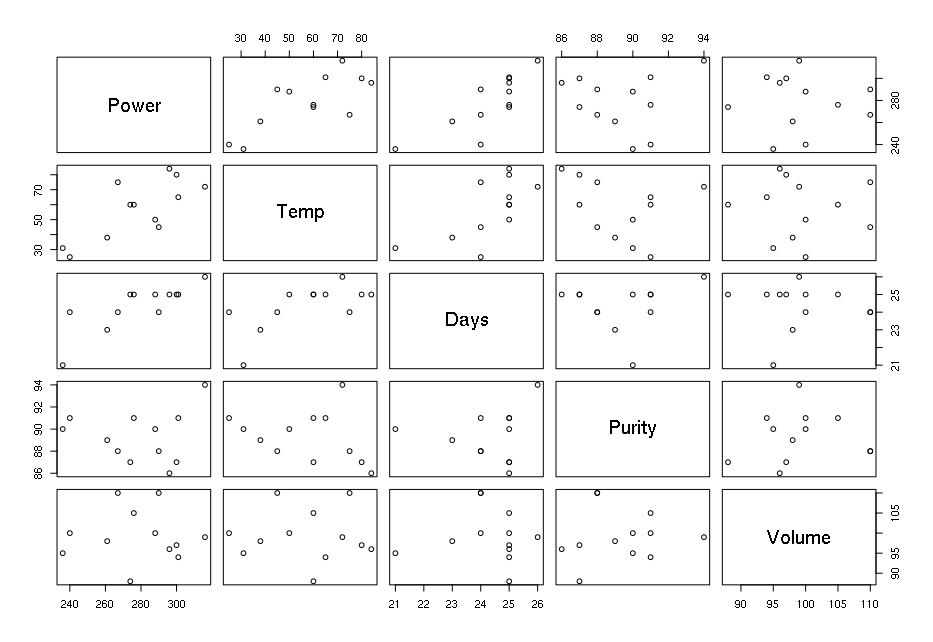
\includegraphics[width=0.8\textwidth]{2a.png}

        There is a clear relationship between power and temperature and
        a slight relationship between power and days. There may be a slight
        relationship between temperature and days.
      \item There is moderately suggestive evidence that at least one variable
        is a significant predictor of power consumption.

        \begin{verbatim}
> # Enter data
> Power = c(240,236,290,274,301,316,300,296,267,276,288,261)
> Temp = c(25,31,45,60,65,72,80,84,75,60,50,38)
> Days = c(24,21,24,25,25,26,25,25,24,25,25,23)
> Purity = c(91,90,88,87,91,94,87,86,88,91,90,89)
> Volume = c(100,95,110,88,94,99,97,96,110,105,100,98)
>
> # Create matrix combine vectors
> data = cbind(Power,Temp,Days,Purity,Volume)
>
> # Plot a scatterplot matrix
> pairs(data)
>
> # Fit a linear model with all for variables
> mod = lm(Power~Temp+Days+Purity+Volume)
> summary(mod)

Call:
lm(formula = Power ~ Temp + Days + Purity + Volume)

Residuals:
    Min      1Q  Median      3Q     Max
-18.758  -9.952   3.350   6.627  23.311 

Coefficients:
              Estimate Std. Error t value Pr(>|t|)
(Intercept) -102.71324  207.85885  -0.494    0.636
Temp           0.60537    0.36890   1.641    0.145
Days           8.92364    5.30052   1.684    0.136
Purity         1.43746    2.39162   0.601    0.567
Volume         0.01361    0.73382   0.019    0.986

Residual standard error: 15.58 on 7 degrees of freedom
Multiple R-squared:  0.7447,  Adjusted R-squared:  0.5989 
F-statistic: 5.106 on 4 and 7 DF,  p-value: 0.0303
        \end{verbatim}
      \item The $R^2$ value of 0.7447 indicates the model fits $74.47\%$ of the
        data.
      \item $\hat{y} = -102.71 + 0.6054(\text{Temp}) + 8.924(\text{Days}) + 1.438(\text{Purity}) + 0.01361(\text{Volume})$
      \item Given all other predictor variables are constant,
        a $1^\circ\text{F}$ change in temperature effects a $0.6054\text{ kW}$
        change in power.
      \item $\hat{y} = -102.71 + 0.6054(50) + 8.924(25) + 1.438(90) + 0.01361(100) = \boxed{281.44\text{ kW}}$
      \item $288-281.44 = \boxed{6.56\text{ kW}}$
      \item \hfill\\
        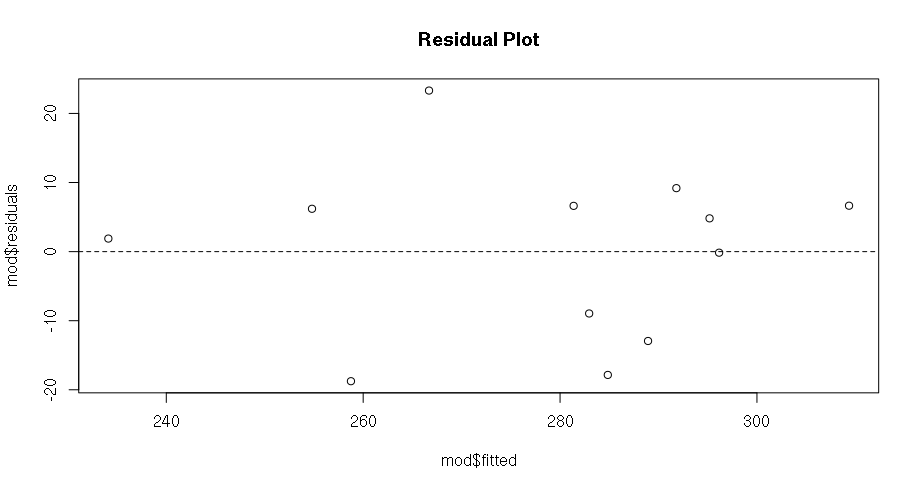
\includegraphics[width=0.8\textwidth]{2h.png}

        There is no pattern in the residual plot, which means the model is not
        leaving out any predictive information, as desired.
    \end{enumerate}

  \item
    \begin{enumerate}
      \item None of the individual variables are significant at the 0.05 level.
      \item The new model depends only on Days as the predictor variable:

        \begin{verbatim}
> mod = lm(Power~Days)
> summary(mod)

Call:
lm(formula = Power ~ Days)

Residuals:
    Min      1Q  Median      3Q     Max 
-33.696  -8.237   4.804  11.353  16.304 

Coefficients:
            Estimate Std. Error t value Pr(>|t|)   
(Intercept)   -90.16      86.74  -1.039  0.32309   
Days           15.16       3.56   4.259  0.00167 **
---
Signif. codes:  0 ‘***’ 0.001 ‘**’ 0.01 ‘*’ 0.05 ‘.’ 0.1 ‘ ’ 1

Residual standard error: 15.38 on 10 degrees of freedom
Multiple R-squared:  0.6446,  Adjusted R-squared:  0.609 
F-statistic: 18.14 on 1 and 10 DF,  p-value: 0.001667
        \end{verbatim}
      \item The model predicts a change of 1 day will effect a 15.16 kW
        increase in power.

        $15.16 \pm t_{0.025,10}(3.56) = 15.16 \pm 2.228(3.56) = \boxed{(7.228,, 23.092)}$

        The 95\% confidence interval estimates the actual increase in power per
        day will be between 7.228 and 23.092 kW.
      \item \hfill\\
        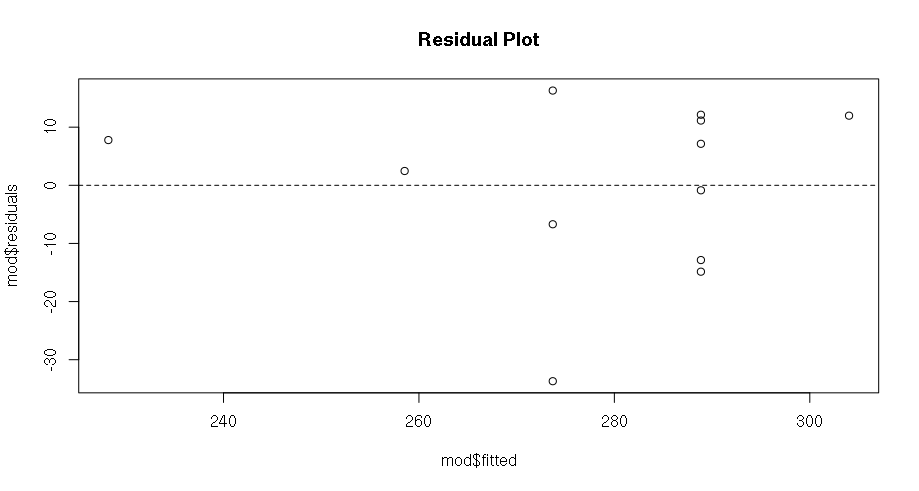
\includegraphics[width=0.8\textwidth]{3d.png}

        There is no pattern in the residual plot, which means the model is not
        leaving out any predictive information, as desired.
      \item $R^2 = 0.6446$ for this model, indicating the model fits 64.46\% of
        the data. This suggests that while Days is a strong predictor of power
        usage, the other predictor variables also have some effect that is not
        accounted for by this new model.
      \item $\hat{y} = -90.16 + 15.16(25) = \boxed{288.84\text{ kW}}$
      \item $288-288.84 = \boxed{-0.84\text{ kW}}$
      \item \hfill\\
        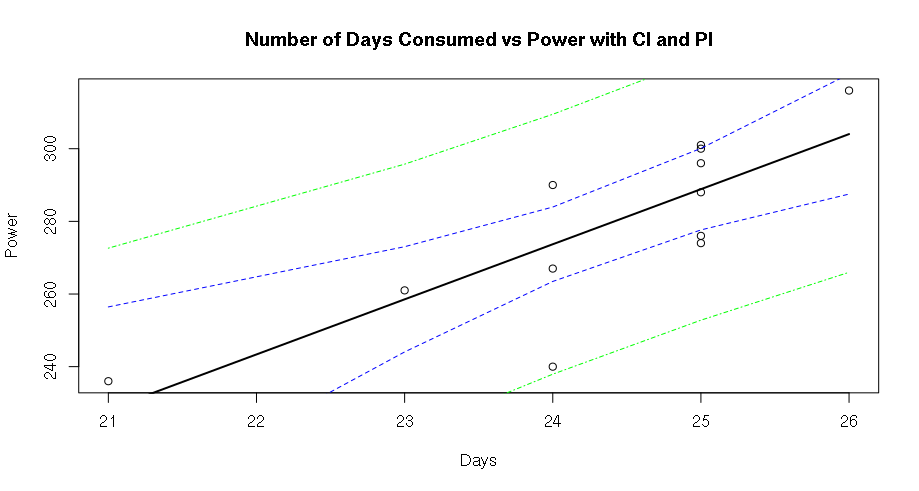
\includegraphics[width=0.8\textwidth]{3h.png}
        % > points(sort(Days), sort(mod$fitted), type="l", lwd=2)
        % > alpha = 0.05
        % > n = length(Days)
        % > df = n-2
        % > SlopeCI = summary(mod)$coefficients[2,1]+c(1,-1)*qt(alpha/2,df)*summary(mod)$coefficients[2,2]
        % > SlopeCI
        % [1]  7.228491 23.092938
        % > SSxx = sum(Days^2)-1/n*sum(Days)^2
        % > MSres = (summary(mod)$sigma)^2
        % > xbar = mean(Days)
        % > ci.bandlow = mod$fitted + qt(alpha/2,df)*sqrt(MSres*(1/n+(Days-xbar)^2/SSxx))
        % > ci.bandhigh = mod$fitted - qt(alpha/2,df)*sqrt(MSres*(1/n+(Days-xbar)^2/SSxx))
        % > pi.bandlow =mod$fitted + qt(alpha/2,df)*sqrt(MSres*(1+1/n+(Days-xbar)^2/SSxx))
        % > pi.bandhigh = mod$fitted - qt(alpha/2,df)*sqrt(MSres*(1+1/n+(Days-xbar)^2/SSxx))
        % > plot(Days,Power, main ="Number of Days Consumed vs Power with CI and PI", xlab="Days", ylab="Power")
      \item 95\% CI: $(277.64, 300.08)$

        The power consumption during 25-day months is, 95\% of the time,
        between 277.64 and 300.08 kW.

        95\% PI: $(252.80, 324.92)$

        The power consumption during a 25-day month can be predicted with 95\%
        confidence to be between 252.80 and 324.92 kW.

        \begin{verbatim}
> xnew=25
> ynew
[1] 288.8571
> ynew+c(1,-1)*qt(alpha/2,df)*sqrt(MSres*(1/n+(xnew-xbar)^2/SSxx))
[1] 277.6393 300.0750
> ynew+c(1,-1)*qt(alpha/2,df)*sqrt(MSres*(1+1/n+(xnew-xbar)^2/SSxx))
[1] 252.7968 324.9175
        \end{verbatim}


    \end{enumerate}
\end{enumerate}

\end{document}

